\externaldocument{../appendix/chapter_app}
\startchapter{Modeling}
\label{chapter:Mod}
In this chapter, I modeled the communication of two running programs. The dual-trace captured from two interacting programs are also modeled in the perspective of communication analysis. The modeling are based on the investigation of some common used communication methods. The communication methods are divided into two categories based on their data transmission properties. This modeling are the foundation to decide how communications being identified from the dual-trace and how to present them to the user. The terminology of using in this chapter can be found in \ref{term}.

\section{Communication Categorization and Communication Methods}
The goal of this work is to identify the communications from the dual-trace. We need to understand the properties of the communications to identify them. In general, there are two types of communication: reliable and unreliable in the terms of their reliability of data transmission. The reason to divide the communication methods into these two categories is that the data transmission properties of the communications fall in different categories affect the mechanism of the data verification in the identification algorithm. In the following two subsections, I summarize the characteristics of these two communication categories. The communication methods list in Table\ref{methodsInCategories} will be discussed further to provide more concrete comprehension. 
\begin{table}[H]
\centering
\caption{Communication Methods Discussed in This Work}
\label{methodsInCategories}
\begin{tabular}{|l|l|}
 \hline
\textbf{Reliable Communication}& \textbf{Unreliable Communication}\\
 \hline
Named Pipes & Message Queue   \\
TCP &  UDP \\
 \hline
\end{tabular}
\end{table}


\subsection{Reliable Communication}\label{reliable}
A reliable communication guarantees the data being sent by one endpoint of the channel is always received losslessly and in the same order in the other endpoint. For some communication methods, a channel can be closed before all sent data being received. With this property, the concatenated data in the receive stream of one endpoint should be the prefix of the concatenated data in the send stream of the other endpoint(potentially equal). Therefore, comparing the concatenated received data of one endpoint to the concatenated sent data of the other can verify the send and receive data.

\subsection{Unreliable Communication}\label{unreliable}
An unreliable communication does not guarantee the data being sent always arrive the receiver. Moreover, the data packets can arrive to the receiver in any order. However, the bright side of unreliable communication is that the packets being sent are always arrived as the origin packet, no data re-segmentation would happen. Accordingly, the send and receive data verification can be done by matching the data packet in a receive event to the data packet in a send event on the other side.

\subsection{Communication Methods}
In this section, I describe the mechanism and the basic data transfer characteristics of each communication method in Table\ref{methodsInCategories} briefly. Moreover, data transfer scenarios are represented correspondingly in diagrams for each communication method. 
 
\subsubsection{Named Pipe}
A named pipe provides FIFO communication mechanism for inter-process communication. It can be a one-way or a duplex pipe. \cite{khambattinamed}

The basic data transfer characteristics of Named Pipe are:
\begin{itemize}
  \item Bytes are received in order
  \item Bytes sent as a segment can be received in multiple segments(the opposite is not true)
  \item No data duplication
  \item If a sent segment is loss, all the following segments will lost(this happen when the receiver disconnect from the channel) 
  
\end{itemize}

Based on these characteristics, the data transfer scenarios of Named pipe can be exemplified in Figure\ref{namedpipe}. 
\begin{figure}[H]
\centerline{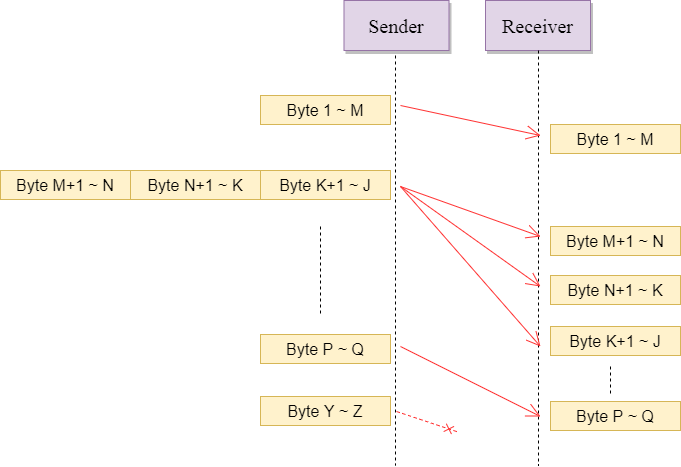
\includegraphics[scale=0.48]{Figures/namedpipe}}
\caption{Data Transfer Scenarios for Named Pipe}
\label{namedpipe}
\end{figure}

\subsubsection{Message Queue}
Message Queuing (MSMQ) is a communication method to allow applications which are running at different times across heterogeneous networks and systems that may be temporarily offline can still communicate with each other. Messages are sent to and read from queues by applications. Multiple sending applications can send messages to and multiple receiving applications can read messages from one queue.\cite{redkar2004pro} In this work, only one sending application versus one receiving application case is considered. Multiple senders to multiple receivers scenario can be divided into multiple sender and receiver situation. Both applications of a communication can send to and receive from the channel.

The basic data transfer characteristics of Message Queue are:
\begin{itemize}
  \item Bytes sent in packet and received in packet, no bytes re-segmented
  \item Packets can lost
  \item Packets received in order
  \item No data duplication
\end{itemize}
Based on these characteristics, the data transfer scenarios of Message Queue can be exemplified in Figure\ref{msmq}.
\begin{figure}[H]
\centerline{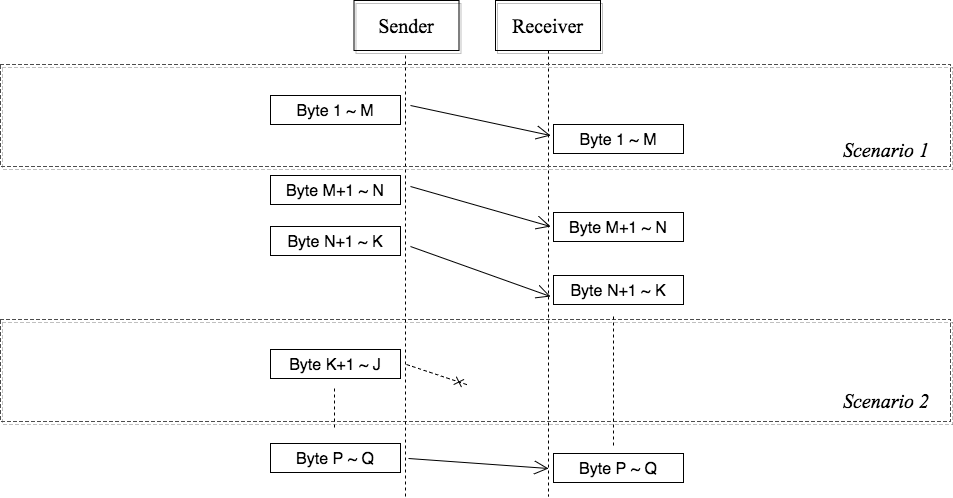
\includegraphics[scale=0.48]{Figures/msmq}}
\caption{Data Transfer Scenarios for Message Queue}
\label{msmq}
\end{figure}

\subsubsection{TCP}
TCP is the most fundamental reliable transport method in computer networking. TCP provides reliable, ordered, and error-checked delivery of a stream of octets between applications running on hosts in an IP network. The TCP header contains the sequence number of the sending octets and the acknowledge sequence this endpoint is expecting from the other endpoint(if ACK is set). The re-transmission mechanism is based on the ACK. 

The basic data transfer characteristics of TCP are:
\begin{itemize}
  \item Bytes received in order
  \item No data lost(lost data will be re-transmitted)
  \item No data duplication
  \item Sender window size is different from receiver's window size, so packets can be re-segmented
\end{itemize}

Based on these characteristics,  the data transfer scenarios of TCP can be exemplified in Figure\ref{tcp}.
\begin{figure}[H]
\centerline{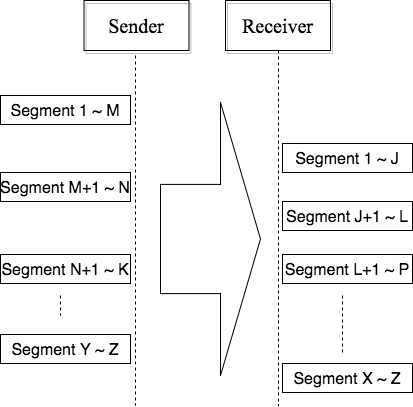
\includegraphics[scale=0.48]{Figures/tcp}}
 \caption{Data Transfer Scenarios for TCP}
\label{tcp}
\end{figure}

\subsubsection{UDP}
UDP is a widely used unreliable transmission method in computer networking. It is a simple protocol mechanism, which has no guarantee of delivery, ordering, or duplicate protection. This transmission method is suitable for many real time systems. 

The basic data transfer characteristics of UDP are:
\begin{itemize}
  \item Bytes sent in packet and received in packet, no re-segmentation
  \item Packets can lost
  \item Packets can be duplicated
  \item Packets can arrive receiver out of order
\end{itemize}

Based on these characteristics, the data transfer scenarios of UDP can be exemplified in Figure\ref{upd}.
\begin{figure}[H]
\centerline{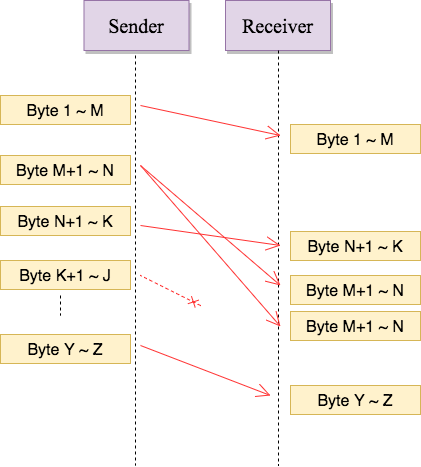
\includegraphics[scale=0.48]{Figures/udp}}
 \caption{Data Transfer Scenarios for UDP}
\label{upd}
\end{figure}

\section{Communication Model}\label{definition}
The communication of two programs is defined in this section. The communication in this work is data transfer activities between two running programs through a specific channel. Some collaborative activities between the programs such as remote procedure call is out of the scope of this research. Communication among multiple programs (more than two) is not discussed in this work. The channel can be reopened again to start new communications after being closed. However, the reopened channel will be treated as a new communication. The way that I define the communication is leading to the communication identification in the dual-trace. So the definition is not about how the communication works but what it looks like. There are many communication methods in the real world and they are compatible to this communication definition. 

\subsection{Communication Definition}
In the context of a dual\_trace, a communication is a sequence of data transmitted between two endpoints through a communication channel. The endpoints connect to each other using the identifier of this channel. We therefore defined a communication c as a triplet:

$c =<ch, e_0, e_1>$

where $e0$ and $e1$ are endpoints while $ch$ is the communication channel used (e.g. a named piped located at /tmp/pipe).

From the point of view of traces, the endpoints $e_0$ and $e_1$ are defined in terms of three properties: the handle created within a process for the endpoint for subsequent operations(e.g. data send and receive), the data stream received and the data stream sent. Therefore, I define an endpoint e as a triplet:

$ e =<handle, d_r, d_s>$

where $d_r$ and $d_s$ are data streams. A data stream is a sequence of events, each sends or receives a package. Each package contains data that is being sent or received (its payload). Hence, we can define a data stream $d$ as a sequence of $n$ packages:

$ d = (pk_1, pk_2, ..., pk_n)$ 

Note that this is the sequence of packages as seen from the endpoint and might be different than the sequence of packages seen in the other endpoint, specially where there is package reordering, loss or duplication.

Each package has several attributes:
\begin{itemize}
\item \textit{Relative time(it was sent or received):} In a trace, we do not have absolute time for an event. However, we know when when an event (i.e. sending or receiving a package) has happened with respect to another event. we will use the notation 

$time(pkg)$ 

to denote this relative time. Hence, if  $i < j $ , then 

$time(pk_i) < time(pk_j)$

\item \textit{Payload:} Each package has a payload (the data being sent). This payload can be modeled as a string contained in the package.we will use the notation 

$pl(pkg)$ 

to denote this payload. 

\end{itemize}


\subsection{Communication Properties}
The properties of the communications can be described based on the definition of the communication.

\subsubsection{Properties of reliable communication:}
A reliable communication guarantees that the data sent and received between a package happens without loss and in the same order.

For a given data stream, I will define the data in this stream as the concatenation of all the payloads of all the packages in this stream, in the same order, and denote is as $data(d)$.

Given $ d = <pk_1, pk_2, ..., pk_n>$, $data(d) = pl(pk_1) \cdot pl(pk_2)\cdot \ldots \cdot pl(pk_n)$


\begin{itemize}
 \item \textit{ Content Preservation:} for a communication:

$c = <ch, <h_0, dr_0, ds_0>, <h_1, dr_1, ds_1>>$

the received data should always be a prefix (potentially equal) of the data sent:

$data(dr_0)$ is a prefix of $data(ds_1)$  and

$data(dr_1)$ is a prefix of $data(ds_0)$

 \item \textit{Timing Preservation:} at any given point in time, the data received by an endpoint should be a prefix of the data that has been sent from the other:
 
for a sent data stream of size $m$, $ds= <pks_1, pks_2, ... pks_m>$ that is received in data stream of size $n$, $dr = <pkr_1, pkr_2, ... pkr_n>$

for any $k \in {1..n}$, there must exist $j \in {1..m}$ such that: $pks_j$ was sent before $pkr_k$ was received:

$  time(pks_j) < time(pkr_k)$

  and

$  data(<pkr_1, pkr_2, ..., pkr_k>)$ is a prefix of $data(<pks_1, pks_2, ..., pks_j>)$

  In other words, at any given time, the recipient can only receive at most the data that has been sent.

\end{itemize}

\subsubsection{Properties of unreliable communication:}
In unreliable communication sender and receiver are not concerned with the concatenation of packages. Instead, they treat each package independent of each other.
\begin{itemize}
 \item \textit{ Content Preservation:} a package that is received should have been sent:

for a sent data stream of size $m$, $ds= <pks_1, pks_2, ... pks_m>$ that is received in data stream of size $n$, $dr = <pkr_1, pkr_2, ... pkr_n>$

for any $pkr_j \in dr$ there must exist $pks_i \in ds$

We will say that the $pkr_j$ is the matched package of $pks_i$, and vice-versa, $pks_i$ is the matched package of $pkr_j$, hence

$match(pkr_j) = pks_i$  and

$match(pks_i) = pkr_j$

 \item \textit{Timing Preservation:}  at any given point in time, packages can only be received if they have been sent

  for a sent data stream of size $m$, $ds= <pks_1, pks_2, ... pks_m>$ that is received in data stream of size $n$, $dr = <pkr_1, pkr_2, ... pkr_n>$

  for any $k \in {1..n}$, $time(match(pkr_j)) < time(pkr_j)$

In other words, the match of the received package must has been sent before it is received.

\end{itemize}



In the following two examples, $h_0$ and $h_1$ are the handles of the two endpoints $e_0$ and $e_1$ of the communications. $ds_0$, $dr_0$ and $ds_1$, $dr_1$ data streams of the endpoints $e_0$ and $e_1$. The string payloads are the strings represented in blue and red in the figures. 

Figure\ref{reliableexample} is an example of the reliable communication. 

\begin{figure}[H]
\centerline{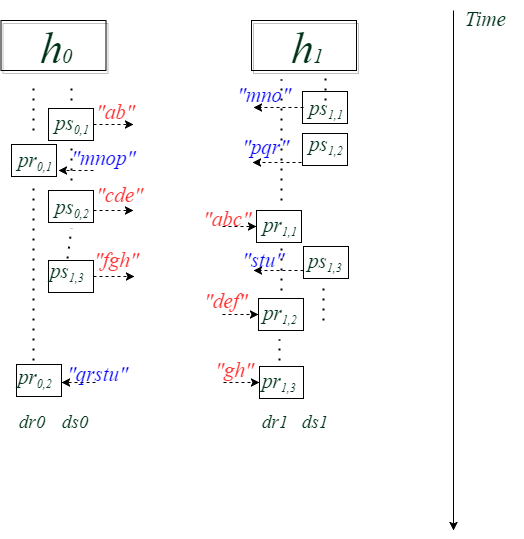
\includegraphics[scale=0.55]{Figures/reliableexample}}
\caption{Example of Reliable Communication}
\label{reliableexample}
\end{figure}

In this example, the payloads of the packages are:

$pl(pks_01)=``ab"$, $ pl(pks_02)=``cde"$, $pl(pks_03)=``fgh"$;

$pl(pkr_11)=``abc"$, $pl(pkr_12)=``def"$, $pl(pkr_13)=``gh"$ .

and 

$pl(pks_11)=``mno"$, $pl(pks_12)=``pqr"$, $pl(pks_13)=``stu"$;

$pl(pkr_01)=``mnop"$, $pl(pkr_02)=``qrstu"$. 

on the other direction. Their properties:

$pl(pks_01) \cdot pl(pks_02) \cdot pl(pks_03) = pl(pkr_11) \cdot pl(pkr_12) \cdot pl(pkr_13) = ``abcdefgh"$ and 

$pl(pks_11) \cdot pl(pks_12) \cdot pl(pks_13) = pl(pkr_01) \cdot pl(pkr_02) = ``mnopqrstu"$. 

satisfy the content preservation. 

The relative time relationship of the packages are: 

$time(pks_01) < time(pks_02) < time(pkr_11)< time(pks_03) < time(pkr_12) < time(pkr_13) $;

$time(pks_11) < time(pks_12) < time(pkr_01)< time(pks_13) < time(pkr_02)$. 

The fact that
 
$pl(pkr_01) = ``mnop"$ is the prefix of $pl(pks_11) \cdot  pl(pks_12) = ``mnopqr"$,

$pl(pkr_01) \cdot pl(pkr_02)=``mnopqrstu"$ is the prefix of(is this case identical to ) $pl(pks_11) \cdot pl(pks_12) \cdot pl(pks_13) = ``mnopqrstu" $,  

$pl(pkr_11)=``abc"$ is the prefix of $pl(pks_01 \cdot pl(pks_02) = "abcde"$,  

$pl(pkr_11) \cdot pl(pkr_12)= ``abcdef"$ and  $pl(pkr_11) \cdot pl(pkr_12) \cdot pl(pkr_13) = ``abcdefgh"$ are  the prefix of  $pl(pks_01) \cdot pl(pks_02) \cdot pl(pks_03)= ``abcdefgh"$

satisfy the timing preservation. 


Figure\ref{unreliableexample} is an example of the unreliable communication. 

\begin{figure}[H]
\centerline{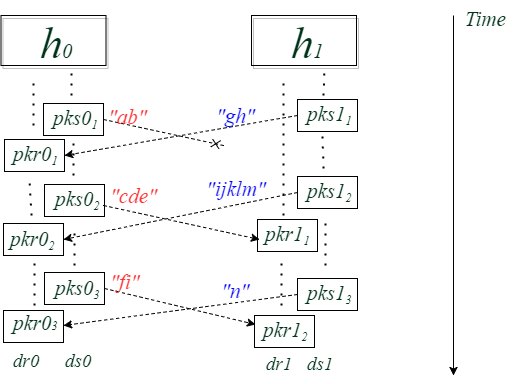
\includegraphics[scale=0.55]{Figures/unreliableexample}}
\caption{Example of Unreliable Communication}
\label{unreliableexample}
\end{figure}

In this example:

$pkr_11 = pks_02=``cde"$, $time(pkr_11) > time(pks_02)$; 

$pkr_12 = pks_02=``cde"$, $time(pkr_12) > time(pks_02)$; 

$pkr_13 = pks_03=``fi"$, $time(pkr_13) > time(pks_03)$;

$pkr_01 = pks_11=``gh"$, $time(pkr_01) > time(pks_11)$;

$pkr_02 = pks_12=``ijklm"$, $time(pkr_02) > time(pks_12)$;

$pkr_03 = pks_13=``n"$, $time(pkr_03) > time(pks_13)$.

All of these satisfy the content preservation and timing preservation of the unreliable communication.


\section{Dual-Trace Model}
Before the modeling, I describe the facts of the dual-trace being analyzed. The traces in a dual-trace are in assembly level. One dual-trace contains two execution traces. There is no timing information of these two traces which means we don't know the time-stamps of the events of these two traces and can not match the events from both sides by time sequence. However the captured instructions in the trace are ordered in execution sequence. The execution traces contain all executed instructions as well as the corresponding changed memory by each instruction. Additionally, system calls are also captured by instruction id, which means if .dll or .exe files are provided, the system function calls can be identified with function names. Memory states can be reconstructed from the recorded memory changes to get the data information of the communication. 

In this model,  a dual\_trace is defined as $dtr = \lbrace tr0, tr1\rbrace$

where $tr0$ and $tr1$ are two assembly execution traces of two interacting programs.

A trace is a sequence of executed instruction line. Hence, we can define a trace $tr$ as a sequence of $n$ lines:

$ tr = (l_1, l_2, ..., l_n)$ 

Each instruction line has three attributes:

\begin{itemize}
\item \textit{Memory changes:}  each assembly instruction has operands which can be register or memory. These operands are being manipulated by the instruction and change the values they hold. The memory changes include all manipulated registers and memories as well as the changed values. we will use the notation 

$mem(l)$ 

to denote this memory changes. 

\item \textit{Function information:} an assembly instruction line might be an entry or return of a function. If it is an entry of a function, it would be able to acquire the function name with presence of the corresponding dynamic libraries. We assume that the function related information can be retrieved by some methods and stored along with the instruction line.

$fun(l)$ 

to denote this function information. 

\item \textit{Line number:} each instruction in a trace is line. The line number of a instruction is the offset of it compare to the first instruction whose line number is 0.

$num(l)$ 

to denote this line number. 

\end{itemize}

From the point of view of the communication analysis, the communications can be recovered by analysis of the relevant function calls(i.e. get the function name, function call line, function return line, input parameters and output parameters) in the traces. This function call can be treated as an event $ev$ and defined as a tripled:

$ev = <funN, sl, el, in, out, type>$

where $funN$ is the function name, $sl$ is the function call line, $el$ is the function return line, $in$ is the input parameters, $out$ is the output parameters and type is the event type which can be one of the four types: channel open, data send, data receive and channel close.

After the definition of event, the trace can be represented in a sequence of events while ignoring all other unconcerned information. This new form of trace is called event trace and defined as $etr$ :

$etr = (ev_1, ev_2, ..., ev_m)$

This event trace is acquired through the processing of the original trace and screen out the concerned function calls. The process to acquire function calls and filter out the relevant ones can be denoted by the notation: 

$etr = eventfilter(tr)$

The events in $etr$ belong to various data streams. The original trace can be also represented as stream trace $str$, which is a set of stream:

$str = \lbrace s_1, s_2, ..., s_p\rbrace$

where $s_i$ is a stream consist of four sub string: channel open stream, data send stream, data receive stream and channel close stream and can be denoted as a tripled:

$s = <so,ss,sr,sc>$

The sub string $sx$ in $s$ consist of a sequence of events which is the sub sequence of $etr$. 

$s = <ev_1, ev_2,..., ev_q>$

Note 1:  the event numbering here is different from the numbering in the $etr$ definition, in another word, $ev_1$ in $s$ is not the same event as $ev_1$ in $etr$. 

Note 2: the events belong to the same sub stream has the same event type. 

A process is used to further distinct them for data streams (i.e. data stream received and the data stream sent) of the corresponding communications, we use the notation:

$str = streamfilter(etr)$

to denote this process.


\section{Relationship between Communication Model and Dual-Trace Model}
The identification of the communication from dual\_trace can be simply abstracted as finding the elements of each communication as defined in the communication model from the dual\_trace. 

A communication is defined as $c =<ch, e0, e1>$ while a dual\_trace is defined as $dtr = \lbrace tr0, tr1\rbrace$. In the dual\_trace model, a trace $tr$ can also be represented as stream trace $str = \lbrace s_1, s_2, ..., s_p\rbrace$. In the communication model, $ e =<handle, d_r, d_s>$. 

Each stream in $str$ contains four sub stream: $so, ss, sr, sc$.  The $handle$ of $e$ and $ch$ in $c$ can be acquired from the events in $so$. $d_r$ can be obtain from $sr$ while $d_s$ can be obtained from $ss$. And $pkg$ in the data stream in the communication model has a one to one relationship with $ev$ in the data send and receive stream in the dual\_trace model.

By understanding this relationship, I am optimistic that as long as I can retrieve all the elements defined in the trace in dual\_trace model, there will be a way to identify the communication. In next chapter algorithms for communication identification will be discussed in detail. 

